\documentclass[svgnames,11pt]{beamer}
\setbeamercolor{structure}{fg=SlateGray}
\usetheme{Goettingen}
\input{/home/tof/Documents/Cozy/latex-include/preambule_commun.tex}
\usepackage{pgfpages}
\setbeameroption{show notes on second screen=left}
\author[]{Christophe Viroulaud}
\title{Chiffrement symétrique}
\date{}
%\logo{}
%\institute{Seconde SNT}
%\institute{Première NSI}
\institute{Terminale NSI}
\setbeamertemplate{navigation symbols}{}
\setbeamertemplate{footline}[frame number]

\begin{document}
\begin{frame}
\titlepage
\end{frame}

\section{Problématique}
\begin{frame}
    \frametitle{Protocole TCP/IP}
La communication sur internet est organisée en couches.
\begin{center}
    \begin{tabular}{|c|}
        \hline
        Couche application (Navigateur)\\
        \hline
        Couche TCP (Transport)\\
        \hline
        Couche IP (Internet)\\
        \hline
        Couche réseau (Matérielle)\\ 
        \hline       
    \end{tabular}
\end{center}
\note[item]{calqué sur le modèle OSI (Open Systems Interconnection)}
\note[item]{Réseau: Définit la forme dont les données sont physiquement transmises quelque soit le réseau (onde, impulsion électrique, lumière)}
\note[item]{IP: Gère les chemins possibles à travers le réseau et achemine le message de l'expéditeur au destinataire.}
\note[item]{TCP: S'assure de la bonne transmission des données. Découpe les messages en paquets.}
\note[item]{Application: Protocole haut-niveau (http, imap\dots)}
\end{frame}
\begin{frame}
    \frametitle{}
En théorie, rien n'interdit à un routeur d'inspecter un paquet et donc d'en connaître son contenu. 
\begin{center}
    \framebox{Comment chiffrer le contenu des communications?}
\end{center}

\end{frame}

\section{Chiffrement symétrique}
\subsection{Principe: le code de César}
\begin{frame}
    \frametitle{Sécurisation: deux étapes}
\begin{itemize}
    \item<1-> La source utilise une \emph{fonction de chiffrement} pour coder un message \emph{m} avec une clé de chiffrement \emph{k}. La fonction produit en sortie un message chiffré \emph{s}.
    \begin{center}
        \textbf{\texttt{chiffrement(m, k) $\rightarrow$ s}}
    \end{center}
    \item<2-> Le destinataire utilise une \emph{fonction de déchiffrement} pour décoder le message \emph{s} avec la clé de chiffrement \emph{k}. La fonction produit en sortie le message clair \emph{m}.
    \begin{center}
        \textbf{\texttt{déchiffrement(s, k) $\rightarrow$ m}}
    \end{center}
\end{itemize}

\end{frame}

\begin{frame}
    \frametitle{}

    \begin{aretenir}[]
        Dans un chiffrement symétrique on utilise la même clé pour chiffrer et déchiffrer le message.
        \end{aretenir}

\end{frame}

\begin{frame}
    \frametitle{}

    \begin{activite}
    Le chiffrement de César utilise un décalage alphabétique comme clé de chiffrement.
    \begin{enumerate}
        \item Écrire la fonction \textbf{\texttt{chiffrement(message: str, cle: int) $\rightarrow$ str}} qui code le \emph{message}. On n'utilisera que des caractères majuscules ASCII dans le message et on supprimera les espaces.
        \item Écrire la fonction \textbf{\texttt{dechiffrement(message: str, cle: int) $\rightarrow$ str}} qui déchiffre le \emph{message}.
        \item Tester la méthode avec une clé $k=+3$ sur le message: \emph{LANSIESTFANTASTIQUE}
        \item Quelles sont les faiblesses de cette méthode?
        %26 possibilités (25) facile à tester tous les cas
    \end{enumerate}
    \end{activite}

\end{frame}
\begin{frame}
    \frametitle{Correction}

\lstinputlisting[firstline=10 ,lastline=14,basicstyle=\small ]{"scripts/cesar.py"}

\end{frame}
\begin{frame}
    \frametitle{Correction}

\lstinputlisting[firstline=17 ,lastline=21,basicstyle=\small ]{"scripts/cesar.py"}

\end{frame}
\begin{frame}[fragile]
    \frametitle{}
    \lstinputlisting[firstline=24 ,lastline=27,basicstyle=\small ]{"scripts/cesar.py"}

    \begin{pycode}
def chiffrement(message: str, cle: int) -> str:
    sortie = ""
    for lettre in message:
        sortie += chr(ord(lettre)+cle)
    return sortie


def dechiffrement(message: str, cle: int) -> str:
    sortie = ""
    for lettre in message:
        sortie += chr(ord(lettre)-cle)
    return sortie


k = 3
entree = "LANSIESTFANTASTIQUE"
m_chiffre = chiffrement(entree, k)
print(m_chiffre)
    \end{pycode}

\end{frame}
\begin{frame}
    \frametitle{Correction}

    Quelle particularité si la clé est 13?
    \note{ROT13}
\end{frame}
\begin{frame}
    \frametitle{Correction}

    Quelle particularité si la clé est 13?
    
    Les fonctions de chiffrement et déchiffrement sont identiques.
\end{frame}
\begin{frame}
    \frametitle{Correction}

    \begin{itemize}
        \item<1->Il n'y a que 25 clés possibles.
        \note[item]{Si on ne prend pas en compte la clé qui transforme en la même lettre.}
        \item<2->La fréquence d'apparition des lettres est une méthode simple à mettre en place pour décrypter un message.
        \begin{center}
        \centering
        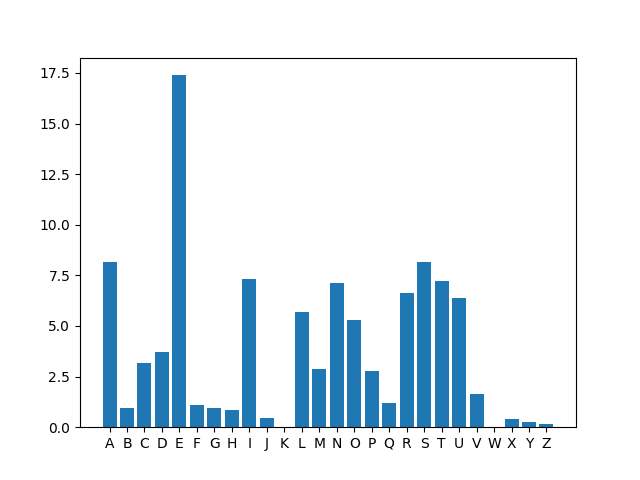
\includegraphics[width=7cm]{ressources/frequence-apparition.png}
        \captionof{figure}{Fréquences d'apparition des lettres \footnote{source: \href{https://www.apprendre-en-ligne.net/crypto/stat/francais.html}{apprendre-en-ligne}}}
        \label{IMG}
        \end{center}
        \note[item]{Si texte est assez long; source: comptage dans une série de 20 livres; \textbf{décryptage:} retrouver le message sans connaître la clé}
    \end{itemize}

\end{frame}
\subsection{Chiffrement polyalphabétique}
\subsubsection{Principe}
\begin{frame}
    \frametitle{Chiffrement polyalphabétique}

    Plutôt que d'opérer un simple décalage, on recopie la clé de chiffrement de façon à obtenir une chaîne de la longueur du message.
\begin{center}
    \begin{tabular}{*{5}{c}}
        B&R&A&V&O\\
        N&S&I&N&S\\
    \end{tabular}
\end{center}
\begin{center}
\textbf{Une même lettre ne sera plus forcément codée par le même symbole.}
\end{center}
\end{frame}

\begin{frame}
    \frametitle{}

    \begin{activite}
        \begin{enumerate}
            \item Remplacer chaque lettre en son équivalent ASCII.
            \item Écrire la fonction \textbf{\texttt{int\_en\_bin(nb: int) $\rightarrow$ str}} qui renvoie la représentation binaire de l'entier \emph{nb}.
            \item Convertir chaque entier en binaire.
        \end{enumerate}
        \end{activite}
\note{on en cache un peu sous le tapis: on est toujours sur 7 bits}
\end{frame}
\begin{frame}
    \frametitle{Correction}

    \begin{center}
        \begin{tabular}{*{5}{c}}
            B&R&A&V&O\\
            66&82&65&86&79\\
            N&S&I&N&S\\
            78&83&73&78&83\\
        \end{tabular}
    \end{center}

\end{frame}
\begin{frame}
    \frametitle{Correction}

    \lstinputlisting[firstline=10 ,lastline=19 ]{"scripts/xor.py"}

\end{frame}
\begin{frame}
    \frametitle{Correction}

    \begin{center}
        \begin{tabular}{*{5}{c}}

            66&82&65&86&79\\
            1000010&1010010&1000001&1010110&1001111\\

            78&83&73&78&83\\
            1001110&1010011&1001001&1001110&1010011\\
        \end{tabular}
    \end{center}

\end{frame}
\subsubsection{Chiffrement par \emph{ou exclusif}}
\begin{frame}
    \frametitle{}
    On applique la porte logique \emph{xor} entre chaque bit du message et de la clé. Une propriété intéressante de cette porte est qu'elle est réversible:
    $$\mbox{Si }A\oplus B = C \mbox{ alors } A\oplus C=B \mbox{ et }B\oplus C=A$$
    \note{vigenere, enigma = substitution polyalphabétique}
    

\end{frame}

\begin{frame}
    \frametitle{}

    \begin{activite}
        \begin{enumerate}
            \item Appliquer le ou exclusif pour chaque bit du message.
            \item Écrire la fonction \textbf{\texttt{bin\_en\_int(paquet: str) $\rightarrow$ int}} qui renvoie l'entier correspondant au paquet de bits.
            \item Utiliser la fonction pour trouver l'entier correspondant à chaque paquet de sept bits.
            \item Donner alors le message chiffré.
            %vérifier qu'on retrouve le message d'origine
        \end{enumerate}
        \end{activite}

\end{frame}
\begin{frame}
    \frametitle{Correction}

    \begin{center}
        \begin{tabular}{*{6}{c}}
            &1000010&1010010&1000001&1010110&1001111\\
            $\oplus$&1001110&1010011&1001001&1001110&1010011\\
            \hline
            &0001100&0000001&0001000&0011000&0011100\\
        \end{tabular}
    \end{center}


\end{frame}

\begin{frame}
    \frametitle{Correction}

    \begin{center}
        \begin{tabular}{*{5}{c}}
            0001100&0000001&0001000&0011000&0011100\\
            12&1&8&24&28\\
        \end{tabular}
    \end{center}
\note{on ne retransforme pas en ASCII: pas d'intérêt et on est sur des caractères non imprimables}
\end{frame}
\section{Avantages du chiffrement symétrique}

\begin{frame}
    \frametitle{Avantages: sûreté}
    Une clé trop courte ne garantit pas une bonne sécurité
    \note[item]{à cause puissance de calculs qui augmentent}
\begin{itemize}
    \item<1-> algorithme DES (\emph{Data Encryption Standard}) obsolète à cause d'une clé maximale de 56 bits.
    \note[item]{$2^{56}$ possibilités; également lenteur pendant le chiffrage}
    \item<2-> algorithme AES: clé 128 bits
    \note[item]{minimum conseillé aujourd'hui: 80 bits}
    \item<3-> Une clé de la taille du message garantit une protection sûre (téléphone rouge).
    \note[item]{montré par Claude Shannon en 1949; père de la théorie de l'information}
    \note[item]{pendant guerre froide (1963): téléphone rouge utilisait une clé de la taille du message}
    
\end{itemize}
    

\end{frame}

\begin{frame}
    \frametitle{Avantages: rapidité}
\begin{itemize}
    \item<1-> Fonctionnement similaire à la méthode du \emph{ou exclusif}.
    \item<2-> \emph{xor} est une fonction implémentée dans les processeurs
    \item <3-> Possibilité de chiffrer en temps réel (données du disque dur par exemple)
\end{itemize}

\end{frame}
\begin{frame}
    \frametitle{Exemples}

    \begin{itemize}
        \item \emph{AES pour Advanced Encryption Standard:} choisi par l'institut de standardisation américain NIST (National Institute of Standards and Technology) en décembre 2001.
        \item \emph{Chacha20:} date de 2008 et améliore les performances d'un autre algorithme (Salsa20)
        \note{20 = étapes de mélange}
    \end{itemize}

\end{frame}

\end{document}